\documentclass{article}

\input{physicsPream}

\usepackage{changepage}

\begin{document}

%----------BEGIN TITLEPAGE----------

\begin{titlepage}

  \title{Lab 5: Spectroscopy}
  \author{Ryan Wojtyla \\
    \textbf{Partners:} \\
    Keefe Kamp \\
    Jacquelyne Miksanek \\
    Akshath Wikramanayake \\
    }
  \date{November 20, 2018}

  \maketitle

  \begin{center}
    Abstract
  \end{center}

  \qq Both of the experiments within this lab involve using the angles of
  diffraction of different bands from a spectrum to calculate the wavelengths of
  the light beams diffracted at those angles. While the calculated values of the
  wavelengths are very near their expected values, relatively small limitations
  of the equipment became extremely large errors after they were propagated
  through the equation relating the diffraction angle to the wavelength.

  \thispagestyle{empty}

\end{titlepage}

%-----------END TITLEPAGE-----------

\section{Experiment 1: Emission Spectrum}

%----------BEGIN EXPERIMENT 1----------

\subsection{Objective}

\qq The purpose of this experiment was to determine the wavelengths of the
colors present in the emission spectrum of mercury vapor. This was accomplished
by shining a beam emitted by mercury vapor through a diffraction grating that
was then rotated. The angles at which each color revealed itself was recorded,
and that angle was used to calculate the wavelength of the colors.

\subsection{Theory}

\qq All the atoms of a particular element have a certain set of discrete
energy levels to which atoms' electrons can be excited. When the electrons fall
back down to their normal positions, a photon with energy equal to one of the
energy levels is emitted. An element's set of energy levels is referred to as
its emission spectrum. 

\qq The energy contained within these energy levels is determined with \(E =
\frac{hc}{\lambda}\). Since \(hc\) is a constant, the energy is dependent solely
upon the wavelength, \(\lambda\), which is the value we are finding in this
experiment. While the wavelength of a particular color cannot be measured
directly, it can be found with

\begin{equation}
  \label{eqn:wavelength}
  \lambda = d \sin{(\lambda)}
\end{equation}

where \(d\) is the distance between the lines of the diffraction grating and
\(\theta\) is the angle of diffraction for a color.

\subsection{Equipment}

\begin{figure}[H]
  \label{tab:equipmentExp1}
  \caption{A list of the equipment used in Experiment 1.}
  \begin{center}
    \begin{tabular}{|c|c|c|c|}
      \hline
      Manufacturer & Model & Serial Number & Specifications \\
      \hline
      PASCO Scientific & Spectrophotometer Kit & OS-8537 & n/a \\
      PASCO Scientific & Aperture Bracket & OS-8534 & n/a \\
      PASCO Scientific & Mercury Spectral Tube & SE-9466 & n/a \\
      PASCO Scientific & Spectral Tube Power Supply & SE-9460 & n/a \\
      PASCO Scientific & Light Sensor & CI-6604 & n/a \\
      PASCO Scientific & Basic Optics Bench & OS-8515 & n/a \\
      PASCO Scientific & Data Acquisition Software & n/a & n/a \\
      \hline
    \end{tabular}
  \end{center}
\end{figure}

\subsection{Procedures}

\qq Since we lacked the Rotary Motion Sensor, the procedures had to be modified
from how they are printed in the manual to include the manual rotating of the
degree plate. 

\qq Once the equipment is set up, rotate the degree plate to
\SI{40}{\degree}. From there, slowly rotate the degree plate until a color
becomes visible on the viewing screen. Record the color and the angle at which
it became revealed, then continue rotating. After the central ray has been
passed, the colors will repeat themselves. Record the negative angle at which
each color reveals itself. This data can be used to calculate the wavelength of
each of the observed colors.

\subsection{Data and Analysis}

\begin{figure}[H]
  \caption{The observed colors, the angles at which they were observed, the
    average of those two angles, and the calculated wavelengths of the colors.}
  \begin{center}
    \begin{tabular}{|c|c|c||c||c|}
      \hline
      Color & \(\theta_1 \pm \SI{0.5}{\degree}\) & 
      \(\theta_2 \pm \SI{0.5}{\degree}\) & \(\theta \pm \SI{0.354}{\degree}\) &
      Wavelength (\si{\nano\meter}) \\       
      \hline
      yellow       & 21   & -19.5 & 20.25 & \(577 \pm 192\) \\ 
      green        & 20   & -17.5 & 18.75 & \(536 \pm 180\) \\ 
      cyan         & 17.5 & -16.5 & 17    & \(487 \pm 163\) \\ 
      purple\(_1\) & 16   & -14   & 15    & \(431 \pm 144\) \\ 
      purple\(_2\) & 14.5 & -13.5 & 14    & \(403 \pm 135\) \\ 
      blue         & 13   & -12.5 & 12.75 & \(368 \pm 123\) \\ 
      \hline
    \end{tabular}
  \end{center}
  \label{tab:exp1data}
\end{figure}

\begin{figure}[H]
  \caption{The known values for the emission spectrum of
    mercury. 
    (\url{https://en.wikipedia.org/wiki/Mercury-vapor\_lamp\#Emission\_line\_spectrum})}
  \begin{center}
    \begin{tabular}{|c|c|}
      \hline
      Color & Wavelength (\si{\nano\meter}) \\
      \hline
      yellow            & 578.2 \\
      green             & 546.1 \\
      blue              & 435.8 \\
      violet            & 404.7 \\
      ultraviolet (UVA) & 365.4 \\
      \hline
    \end{tabular}
  \end{center}
  \label{tab:exp1known}
\end{figure}

\qq The goal of this experiment was to calculate the wavelength of the observed
colors using only the known value of the diffraction slit distance, \(d =
\SI{1666}{\nano\meter}\), and the measured values of the angles at which the
colors appeared with Equation \ref{eqn:wavelength}. The first step was to record
the two angles, positive and negative, at which each color appeared. This data is
shown in the first section of Figure \ref{tab:exp1data}. 

\qq Now that two raw angles for each color have been found, their average must
be taken to obtain one value for each color's angle. This is done using the
classic average formula \(\theta = \frac{|\theta_1| + |\theta_2|}{2}\). The
calculation for the color yellow is shown:

\begin{align*}
  \theta                 &= \frac{\left| \theta_1 \right| + \left| \theta_2
                           \right|}{2} \\
  \theta_{\text{yellow}} &= \frac{\left| (21) \right| + \left| (-19.5)
                           \right|}{2} \\
  \theta_{\text{yellow}} &= \SI{40.5}{\degree} \\
\end{align*}

\qq Since all the colors' angle measurements share a common error, the error of
the average of the two measurements is uniform across the colors, therefore, it
only need be calculated once. Since \(\theta\) is calculated by dividing the sum
of \(\theta_1\) and \(\theta_2\) by a constant, \(2\), the error of \(\theta\),
\(\delta \theta\), can be calculated with:

\begin{align*}
  \delta\theta &= \frac{1}{2} \sqrt{\delta\theta_1 ^ 2 + \delta\theta_2 ^2} \\
  \delta\theta &= \frac{1}{2} \sqrt{(0.5)^2 + (0.5)^2} \\
  \delta\theta &= \SI{0.354}{\degree} \\
\end{align*}

\qq The average angles at which each color was found is shown in the second
section of Figure \ref{tab:exp1data}.

\qq The wavelengths of the colors can be calculated with
\(\lambda(\theta) = d \sin{(\theta)}\), where \(d = \SI{1666}{\nano\meter}\) is
the distance between the slits of the diffraction grating and \(\theta\) is the
angle at which the color was found. The calculation for the color yellow is
shown:

\begin{align*}
  \lambda_{\text{yellow}} &= d \sin{(\theta_{\text{yellow}})} \\
  \lambda_{\text{yellow}} &= (\num{1666e-9}) \sin{(20.25)} \\
  \lambda_{\text{yellow}} &= \SI{577}{\nano\meter} \\
\end{align*}

\qq In order to determine the propagation of error through a function with one
variable, the derivative of that function must be found then multiplied by the
accepted value of the function and the error of the value to be
propagated. Therefore, the error of the wavelength, \(\delta\lambda\), can be
found with

\begin{align*}
  \delta\lambda &= \lambda \frac{d \lambda}{d \theta} \delta\theta \\
  \delta\lambda &= \lambda (\cos{(\theta)}) \delta\theta \\
\end{align*}

Again, the calculation for the color yellow will be shown as the example

\begin{align*}
  \delta\lambda_{\text{yellow}} &= \lambda_{\text{yellow}}
                                  \cos{(\theta_{\text{yellow}})} \delta\theta \\
  \delta\lambda_{\text{yellow}} &= (\num{577e-9}) \cos{(20.25)} (0.354) \\
  \delta\lambda_{\text{yellow}} &= \SI{192}{\nano\meter} \\
\end{align*}

\qq The results of the other colors are recorded in the third column of Figure
\ref{tab:exp1data}.  

\subsection{Conclusion}

\qq While the uncertainty in the calculated wavelengths is quite high, the
values of the wavelengths are very near their known values, listed in Figure
\ref{tab:exp1known}! The high degree of uncertainty is due to the lack of
precision in our ability to measure the angle at which the colors
appeared. Since the degree table only had increments of \SI{1}{\degree}, the
uncertainty for the degree measurements had to be \(\pm \SI{0.5}{\degree}\),
which propagated quite heavily through the calculations.

%-----------END EXPERIMENT 1-----------

\section{Experiment 2: Absorption Spectrum}

%----------BEGIN EXPERIMENT 2----------

\subsection{Objective}

\qq The purpose of this experiment was to determine the sodium-emitted
wavelengths absorbed by a red liquid sample. This was accomplished by first
measuring the absorption spectrum of sodium through an empty cuvette, then
measuring the spectrum again through a cuvette containing the sample. These two
spectra can be compared to determine which wavelengths were absorbed by the
liquid.

\subsection{Theory}

\qq The fundamental theory behind Experiment 2 is similar to that of Experiment
1; the angles of particular regions of interest are used to find the wavelength
of light in those regions with Equation \ref{eqn:wavelength}. How those regions
of interest are identified, however, is the opposite from Experiment 1. In
Experiment 1, the regions of interest were where light was present, but in
Experiment 2, those regions are where light is absent. By measuring the angles
of these dark regions, the wavelengths of absorbed light can be calculated.

\qq A base spectrum is first determined by measuring the emission spectrum of
the sodium sample through a blank cuvette. This base is then compared to the
spectrum of the sample shone through a cuvette filled with a sample. The
difference between the two spectra, the angles at which the filled cuvette's
spectrum is of lower intensity than the blank cuvette's, represents the
absorption spectrum of the sample in the filled cuvette.

\subsection{Equipment}

\begin{figure}[H]
  \label{tab:equipmentExp2}
  \caption{A list of the equipment used in Experiment 2.}
  \begin{center}
    \begin{tabular}{|c|c|c|c|}
      \hline
      Manufacturer & Model & Serial Number & Specifications \\
      \hline
      PASCO Scientific & Spectrophotometer Kit & OS-8537 & n/a \\
      PASCO Scientific & Aperture Bracket & OS-8534 & n/a \\
      PASCO Scientific & Sodium Spectral Tube & SE-9466 & n/a \\
      PASCO Scientific & Spectral Tube Power Supply & SE-9460 & n/a \\
      PASCO Scientific & Light Sensor & CI-6604 & n/a \\
      PASCO Scientific & Basic Optics Bench & OS-8515 & n/a \\
      PASCO Scientific & Data Acquisition Software & n/a & n/a \\
      n/a              & Cuvette & n/a & x2 \\
      n/a              & Red Colored Liquid & n/a & \SI{5}{\milli\liter} \\
      \hline
    \end{tabular}
  \end{center}
\end{figure}

\subsection{Procedures}

\qq The procedures for Experiment 2 are very similar to that of Experiment
1. Again, since we lacked the Rotary Motion Sensor, the procedures printed here
differ from the lab manual in that we had to manually rotate the degree plate
and record the intensity of the beam at each angle.

\qq Once the equipment is set up as it was in Experiment 1, place the blank
cuvette into the holder between the diffraction grating and the light intensity
sensor. Set up the software for the light intensity sensor. Begin by rotating
the degree plate to \SI{-40}{\degree} and recording the intensity of the light in
the data acquisition software. From there, rotate the degree plate in increments
of one degree and record the intensity in the software for each angle up to
\SI{40}{\degree}. Save the data, reset the data acquisition software, replace
the blank cuvette with the one containing the sample, and repeat the data
acquisition process.

\subsection{Data and Analysis}

\begin{figure}[H]
  \label{gph:exp2data}
  \begin{adjustwidth}{-5cm}{}
    \begin{center}
      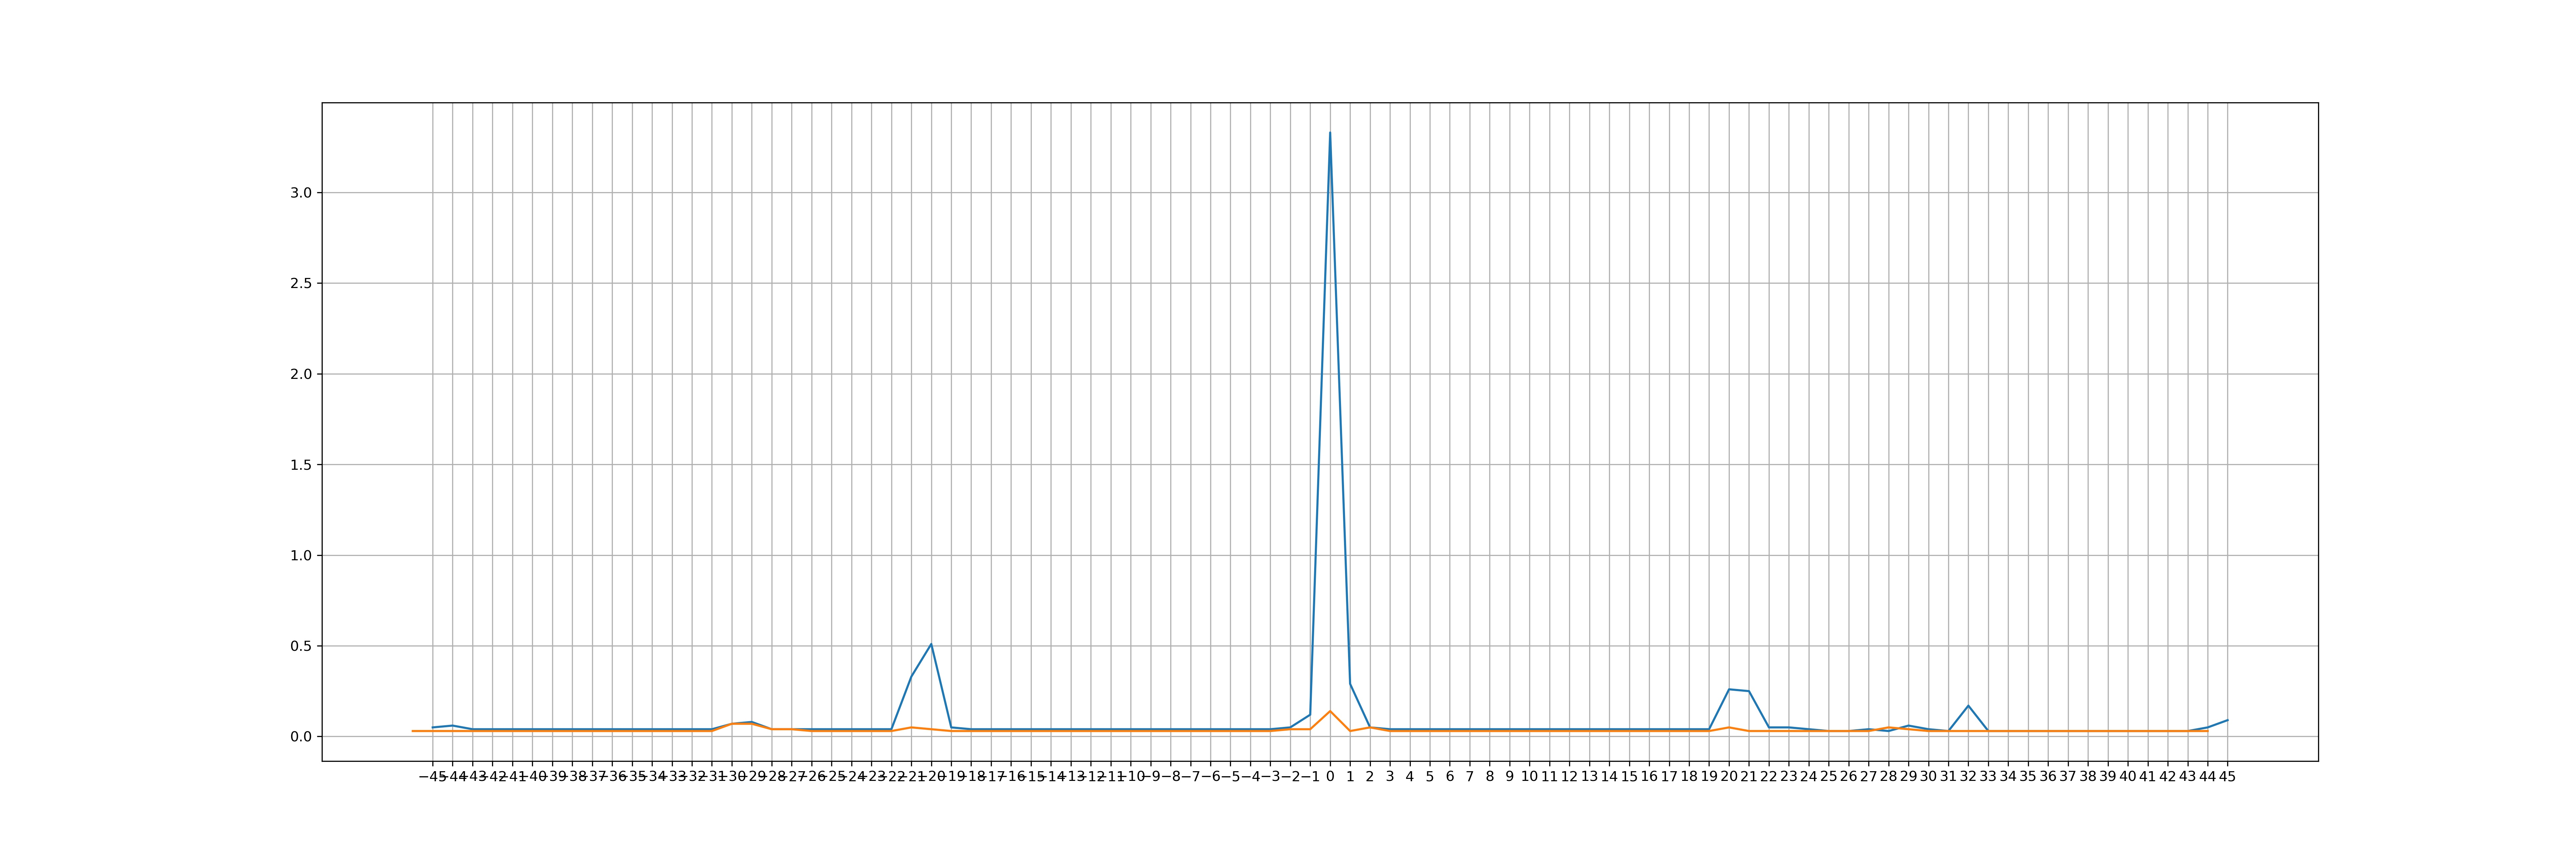
\includegraphics[scale=0.35]{exp2.jpg}
    \end{center}
  \end{adjustwidth}
  \caption{A plot of the Intensity (y-axis) as the Angle of the Degree Plate
    (x-axis) changes. The blue line is the intensity of the blank cuvette, and
    the orange line is the intensity of the filled cuvette.}
\end{figure}

\qq Before calculations can be performed the graph must first be analyzed to
identify the angles at which the sample absorbed the incident light. This is
accomplished by noting where the blue line peaks and the orange line remains
flat. This requirement automatically omits the central ray since the orange line
also peaks, albeit at a far lower intensity, when \(\theta =
\SI{0}{\degree}\). 

\qq Additionally, in order to verify the authenticity of the data, both the
negative and positive angle ranges were recorded. Since the peaks ought to
mirror each other, any errors will be quickly identifiable because anomalies
will not have a twin peak on the opposite side of the central ray. This
validation requirement can be applied to the peak at \(\theta =
\SI{32}{\degree}\), which does not have a matching twin near \(\theta =
\SI{-32}{\degree}\).  

\qq After all the limitations have been applied, the only two peaks of interest
appear at \(\theta_1 = \SI{-20}{\degree}\) and \(\theta_2 =
\SI{20}{\degree}\). Because the smallest increment of measurement on the degree
plate is \SI{1}{\degree}, the two angle measurements share an error of
\(\delta\theta_1 = \delta\theta_2 = \pm \SI{0.5}{\degree}\). 

\qq The wavelength of the light absorbed by the sample at \(\theta = \pm
\SI{20}{\degree}\) can be calculated using the same method as Experiment 1,
using \(\lambda = d \sin{(\theta)}\), where \(d = \SI{1666}{\nano\meter}\). 

\qq Since \(|\theta_1| = |\theta_2|\), there is no need to find the average
between the two, \(\theta = \SI{20}{\degree}\). The error, however, does need to
be calculated. Since the errors are the same as in Experiment 1,
\(\delta\theta\) in Experiment 2 equals \(\delta\theta\) from Experiment
1. Therefore, \(\delta\theta = \SI{0.354}{\degree}\).

\qq Now that the angle has been finalized to be \(\theta = \SI{20}{\degree}\),
the wavelength of the absorbed light can be found,

\begin{align*}
  \lambda &= d \sin{(\theta)} \\
  \lambda &= (\num{1666e-9}) \sin{(20)} \\
  \lambda &= \SI{570}{\nano\meter} \\
\end{align*}

The error in the wavelength is also calculated the same as in Experiment 1,

\begin{align*}
  \delta\lambda &= \lambda \cos{(\theta)} \delta\theta \\
  \delta\lambda &= (\num{570e-9}) \cos{(20)} (0.354) \\
  \delta\lambda &= \SI{190}{\nano\meter} \\
\end{align*}

The wavelength of the absorbed light is \(570 \pm \SI{190}{\nano\meter}\),
yellow.

\subsection{Conclusion}

\qq As in Experiment 1, while the error in the calculated wavelength is quite
high, the found value is near what is expected. Again, this high uncertainty is
due to limitations present in the equipment itself, namely, the relatively low
precision of the markings on the degree table.

%-----------END EXPERIMENT 2-----------

\end{document}
